\section{Contribution \& validation}
%\label{sec:intro:contrib}

%In this thesis, we argue that modern modelling frameworks should consider uncertainty and time as first-class concepts.
%In this dissertation, I present two contributions that support this vision.
%First, we define a language with uncertainty at a first-class citizen: \langName.
%We detail this contribution in~\Cref{chapt:aintea}.
%Second, we define a \gls{metamodel}, and we formalise it, of the knowledge of \glspl{adptSyst}.
%We present this contribution in~\Cref{chapt:tkm}.
%
Dans cette thèse, nous soutenons que les cadres de modélisation modernes devraient considérer l'incertitude et le temps comme des concepts de première classe.
Dans ce mémoire, je présente deux contributions qui appuient cette vision.
Tout d'abord, nous définissons une langue avec incertitude chez un citoyen de première classe : \langName. 
%Nous détaillons cette contribution au~\Cref{chapt:aintea}. 
Deuxièmement, nous définissons un métamodèle, et nous le formalisons, de la connaissance des systèmes adaptatifs. 
%Nous présentons cette contribution au~\Cref{chapt:tkm}.

\paragraph{\langName{}: Gérer l'incertitude des données au niveau du language}
\begin{figure}
	\centering
	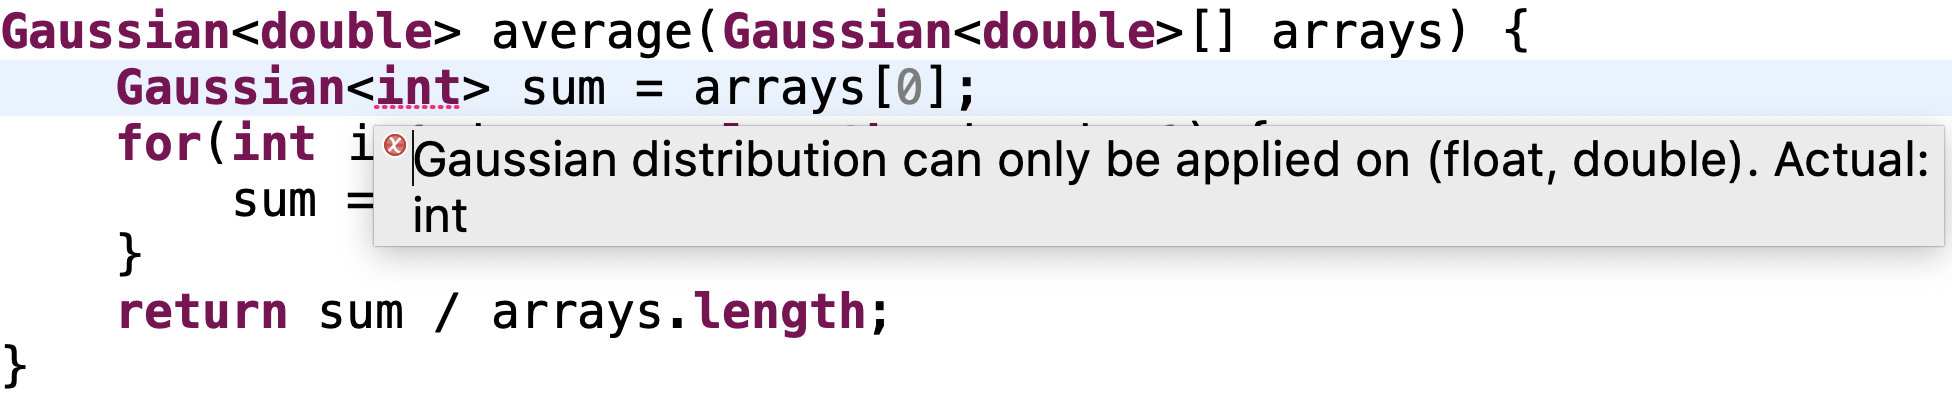
\includegraphics[width=\linewidth]{img/chapt-intro/approach/aintea-overview}
	\caption{Overview of the language proposed, \langName{}}
	\label{fig_french_contrib_aintea}
\end{figure}

%This contribution addresses the challenge of the manipulation of uncertain data (cf. Sub-Challenge \#1). 
%We propose \langName{}, a language able to represent uncertain data as built-in language types along with their supported operations.
%An overview of the language is depicted in~\Cref{fig:french:contrib:aintea}.
% It contains a sampling of distributions (Gaussian, Bernoulli, binomial, Dirac delta function, and Rayleigh) that covers the different data types (booleans, numbers, and references).
% We implement a prototype of the language, publicly available on GitHub\footnote{\url{https://github.com/lmouline/aintea/}}.
% We use a real-world case study based on \gls{sg}, built with our partner Creos S.A..
%It shows first that our approach does not impact the conciseness of the language.
%Second, it highlights the feasibility and the advantages of uncertainty-aware type checking systems on the language level.
%
Cette contribution aborde le défi de la manipulation des données incertaines (cf. Sous-défi \#1). 
Nous proposons \langName{}, un langage capable de représenter des données incertaines comme des types de données intégrés au language avec leurs opérations supportées. 
La~\cref{fig_french_contrib_aintea} donne un aperçu du langage utilisé. 
Il contient un échantillon des lois de probabilités (Gaussiennes, Bernoulli, binomiales, Rayleigh, et la fonction delta de Dirac) qui couvre les différents types de données (booléens, nombres et références). 
Nous avons implémenté un prototype du langage, disponible publiquement sur GitHub\footnote{\url{https://github.com/lmouline/aintea/}}. 
Nous utilisons une étude de cas basée sur un réseau intelligent, réalisée avec notre partenaire Creos S.A.. 
L'évaluation montre d'abord que notre approche n'a pas d'impact sur la concision de la langue. 
Deuxièmement, elle souligne la faisabilité et les avantages des systèmes de contrôle de type sensibles à l'incertitude au niveau linguistique.

%This contribution is under submission at the JOT Journal\footnote{\url{http://www.jot.fm/}}:
%\begin{itemize}
%	\item \citetitle{insubmission:2019:comlan:datauncertainty}, \citeauthor{insubmission:2019:comlan:datauncertainty}
%\end{itemize}
%
Cette contribution a été soumise au journal JOT\footnote{\url{http://www.jot.fm/}} :
\begin{itemize}
	\item \citetitle{insubmission:2019:comlan:datauncertainty}, \citeauthor{insubmission:2019:comlan:datauncertainty}
\end{itemize}

\paragraph{Un métamodèle temporel de la connaissance}
\begin{figure}
	\centering
	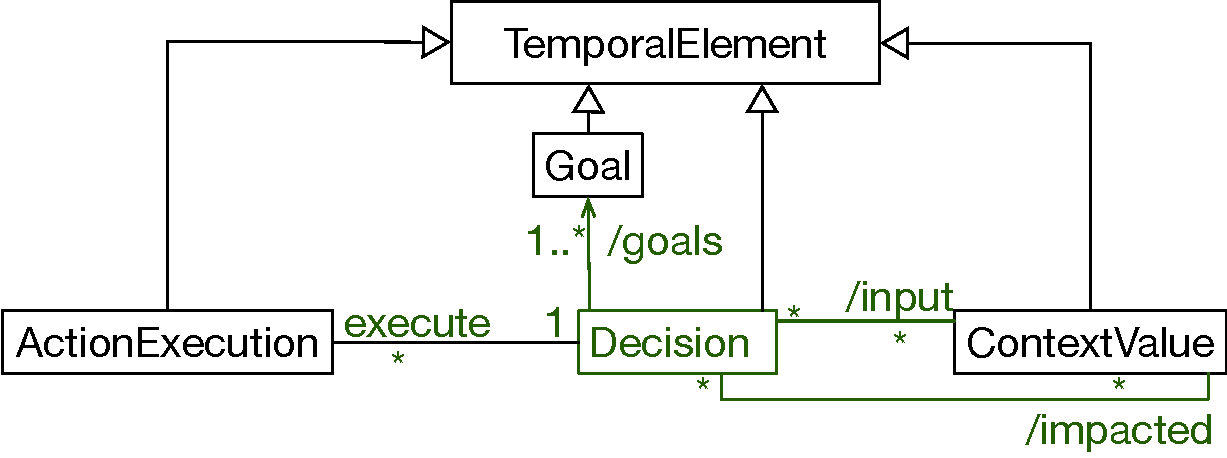
\includegraphics[width=0.6\linewidth]{img/chapt-intro/approach/tkm-overview}
	\caption{Overview of the temporal knowledge model}
	\label{fig_french_contrib_tkm}
\end{figure}

%This contribution addresses the challenge of reasoning over unfinished actions, and understanding of \gls{adptSyst} \gls{behaviour} (cf. Sub-Challenge \#2 and \#3).
%First, we formalise the common core concepts implied in adaptation processes, also referred to as \gls{knowledge}.
%The formalisation is based on temporal graphs and a set of relations that trace decision impacts to circumstances.
%Second, we propose a framework to structure and store the state and behaviour of a running \gls{adptSyst}, together with a high-level \gls{api} to efficiently perform diagnosis routines.
%Our framework relies on a temporal model-based solution that efficiently abstracts decisions, their corresponding circumstances, and their effects.
%We give an overview of the \gls{metamodel} in~\Cref{fig:french:contrib:tkm}.
%We demonstrate the applicability of our approach by applying it to a \gls{sg} based example.
%We also show that our approach can be used to diagnose the behaviour of at most the last five days of a district in the Luxembourg \gls{sg} in $\sim$2.4 seconds.
%
Cette contribution aborde le défi du raisonnement sur les actions inachevées et de la compréhension du comportement des systèmes adaptatifs (cf. Sous-défi \#2 et \#3). 
Tout d'abord, nous formalisons les concepts de base communs impliqués dans les processus d'adaptation, également appelés connaissances. 
La formalisation est basée sur des graphes temporels et un ensemble de relations qui retracent l'impact des décisions sur les circonstances. 
Deuxièmement, nous proposons un \textit{framework} pour structurer et stocker l'état et le comportement d'un système adaptatif en fonctionnement, ainsi qu'une API de haut niveau pour effectuer efficacement des routines de diagnostic. 
Notre \textit{framework} s'appuie sur une solution basée sur un modèle temporel qui résume efficacement les décisions, leurs circonstances correspondantes et leurs effets. 
Nous donnons un aperçu du métamodèle dans la~\cref{fig_french_contrib_tkm}. 
Nous démontrons l'applicabilité de notre approche en l'appliquant à un exemple basé sur un réseau intelligent. 
Nous montrons également que notre approche peut être utilisée pour diagnostiquer le comportement d'au plus les cinq derniers jours d'une période de sur le réseau intelligent luxembourgeois en $\sim$2.4 secondes.

%Part of this contribution has been published at the IEEE International Conference on Autonomic Computing\footnote{\url{http://icac2018.informatik.uni-wuerzburg.de/}} (ICAC) and at the ACM/SIGAPP Symposium On Applied Computing\footnote{\url{http://www.sigapp.org/sac/sac2018/}} (SAC):
%\begin{itemize}
%	\item \citetitle{DBLP:conf/sac/MoulineB0FBMB18}, \citeauthor{DBLP:conf/sac/MoulineB0FBMB18}
%	\item \citetitle{DBLP:conf/icac/MoulineBFBB18}, \citeauthor{DBLP:conf/icac/MoulineBFBB18}
%\end{itemize}
%
Une partie de cette contribution a été publiée à la conférence internationale de l'IEEE.
sur l'informatique autonome\footnote{\url{http://icac2018.informatik.uni-wuerzburg.de/}} (ICAC) et au Symposium ACM/SIGAPP sur l'informatique appliquée\footnote{\url{http://www.sigapp.org/sac/sac2018/}} (SAC) :
\begin{itemize}
	\item \citetitle{DBLP:conf/sac/MoulineB0FBMB18}, \citeauthor{DBLP:conf/sac/MoulineB0FBMB18}
	\item \citetitle{DBLP:conf/icac/MoulineBFBB18}, \citeauthor{DBLP:conf/icac/MoulineBFBB18}
\end{itemize}


